\section{Residual Connections and U-Net}
\begin{frame}{}
    \LARGE Image Segmentation: \textbf{Residual Connections and U-Net}
\end{frame}

\begin{frame}{Can We Do Better?}
\begin{itemize}
    \item The downsampling-then-upsampling approach works well for semantic segmentation.
    \item \textbf{But... can we do better?}
    \item \textbf{Problem}: Important details and spatial information may be lost during downsampling.
    \pause
    \item \textbf{Solution}: Introduce \textbf{residual connections} to preserve spatial information.
\end{itemize}
\end{frame}

\begin{frame}{Residual Connections in Segmentation}
\begin{itemize}
        \item Directly connect features from downsampling layers to upsampling layers.
        \item Help recover lost spatial details and improve segmentation accuracy.
    \begin{figure}
    \centering
    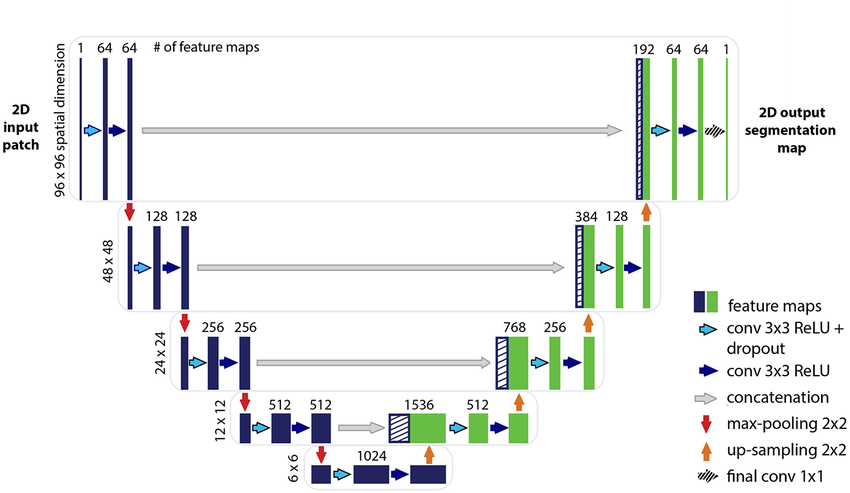
\includegraphics[width=1.0\textwidth,height=0.7\textheight,keepaspectratio]{images/segmentation/Unet.png}
    \end{figure}
\end{itemize}
\end{frame}

\begin{frame}{Residual Connections in Segmentation}
\begin{itemize}
    \item There are two Types of Residuals:
    \begin{itemize}
        \item \textbf{Addition:} Adds features from the encoder to the decoder \textbf{element-wise}.
        \item \textbf{Concatenation:} Concatenates features from the encoder to the decoder along the \textbf{channel dimension}.
    \end{itemize}
    \item \textbf{Which Is Better?}
    \begin{itemize}
        \item Concatenation is often better because it retains more feature information from the encoder.
        \item \textbf{Note}: technically, concatenation might be harder to implement because it requires aligning input and output shapes.
    \end{itemize}
\end{itemize}
\end{frame}

\begin{frame}{U-Net}
\begin{itemize}
    \item This architecture, with residual connections, is called \textbf{U-Net}.
    \item \textbf{Why the name?}
    \begin{itemize}
        \item The architecture resembles the shape of the letter "U".
        \item Features are downsampled in the encoder and upsampled in the decoder, with skip connections in between.
    \end{itemize}
    \item U-Net is widely used for segmentation tasks, especially in biomedical imaging.
\end{itemize}
\begin{figure}
    \centering
    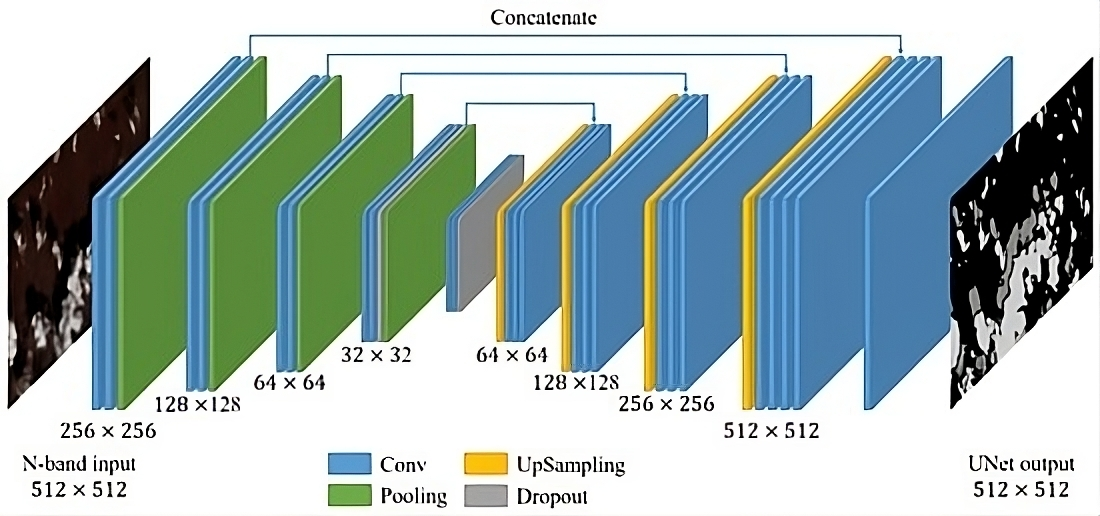
\includegraphics[width=0.75\linewidth]{images/segmentation/unet2.jpeg}
\end{figure}
\end{frame}

\begin{frame}{Using a Pretrained U-Net}
\begin{itemize}
    \item \textbf{Pretrained Encoder:}
    \begin{itemize}
        \item The encoder can use a pretrained backbone (e.g., ResNet, EfficientNet).
        \item This help utilize features learned on large datasets (e.g., ImageNet).
        \item Only the decoder is trained from scratch for segmentation-specific tasks.
    \end{itemize}
    \begin{figure}
    \centering
    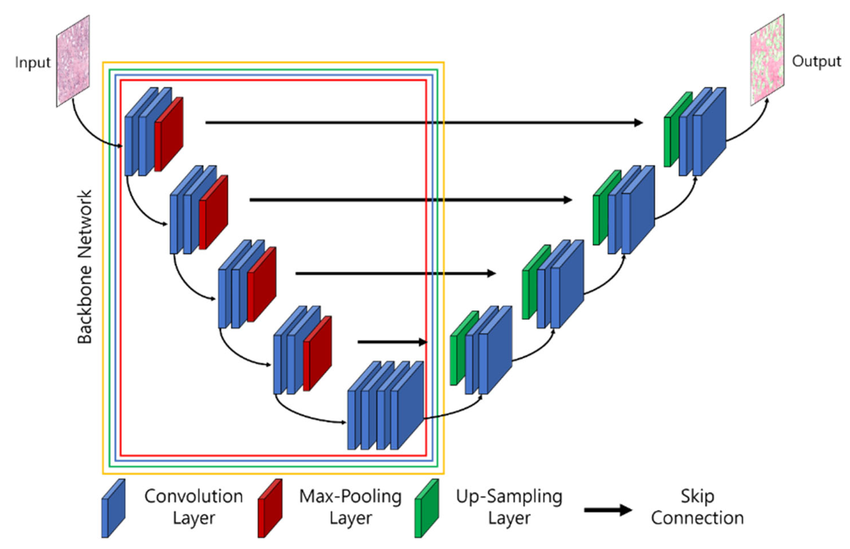
\includegraphics[width=0.75\linewidth]{images/segmentation/pretrained_unet.png}
    \end{figure}
\end{itemize}
\end{frame}
